\section[تمرین دوم - سؤال اول: کاهش بعد با PCA و LDA]
{\faProjectDiagram\ \ تمرین دوم ـ سؤال اول: پیاده‌سازی دستی و کتابخانه‌ای روش‌های کاهش بعد PCA و LDA}

\begin{stepbox}

\field{هدف و معرفی مسئله}{
هدف این بخش، پیاده‌سازی الگوریتم‌های **تحلیل مؤلفه‌های اصلی (\lr{PCA})** به عنوان یک روش کاهش بعد بدون نظارت (\lr{Unsupervised}) و **تحلیل ممیز خطی (\lr{LDA})** به عنوان یک روش با نظارت (\lr{Supervised}) بر روی مجموعه داده دیابت (\lr{diabetes.csv}) می‌باشد.

در این سؤال، نحوه عملکرد الگوریتم‌ها با پیاده‌سازی ریاضی دستی توسط کتابخانه \lr{NumPy} انجام شده و خروجی‌های بصری آن به صورت دقیق با خروجی‌های کتابخانه \lr{Scikit-Learn} مقایسه و تحلیل گردید.
}

\field{پیش‌پردازش داده‌ها و استانداردسازی}{
مجموعه داده دیابت شامل ۷۶۸ نمونه و ۸ ویژگی پزشکی (مانند قند خون، انسولین، فشار خون و سن) به همراه متغیر هدف \lr{Outcome} است.

از آنجا که روش‌های کاهش بعد مبتنی بر ماتریس کواریانس و فاصله‌ها هستند، ویژگی‌ها با استفاده از \lr{StandardScaler} به میانگین صفر و واریانس یک استانداردسازی شدند:

\[
z = \frac{x - \mu}{\sigma}
\]
}

\field{پیاده‌سازی دستی الگوریتم PCA و LDA}{
مراحل پیاده‌سازی ریاضی دو الگوریتم با \lr{NumPy} به شرح زیر انجام شد:

\begin{itemize}
\item **الگوریتم PCA:** با مرکزیک کردن داده‌ها، محاسبه ماتریس کواریانس و استخراج بردارهای ویژه (\lr{Eigenvectors})، ۲ مؤلفه اصلی برتر انتخاب شدند.
\item **الگوریتم LDA:** با محاسبه ماتریس‌های پراکندگی درون‌کلاسی ($\mathbf{S}_W$) و بین‌کلاسی ($\mathbf{S}_B$) و حل مسئله مقدار ویژه تعمیم‌یافته برای $\mathbf{S}_W^{-1} \mathbf{S}_B$ پیاده‌سازی شد. با توجه به $C=2$ کلاس، خروجی LDA به $C-1=1$ بعد نگاشت گردید.
\end{itemize}
}

\field{تحلیل بصری خروجی‌ها و مقایسه پیاده‌سازی‌ها}{
با بررسی دقیق چهار نمودار تولیدشده در خروجی کد، نتایج تحلیلی زیر استخراج گردید:

\vspace{0.4cm}

\begin{center}
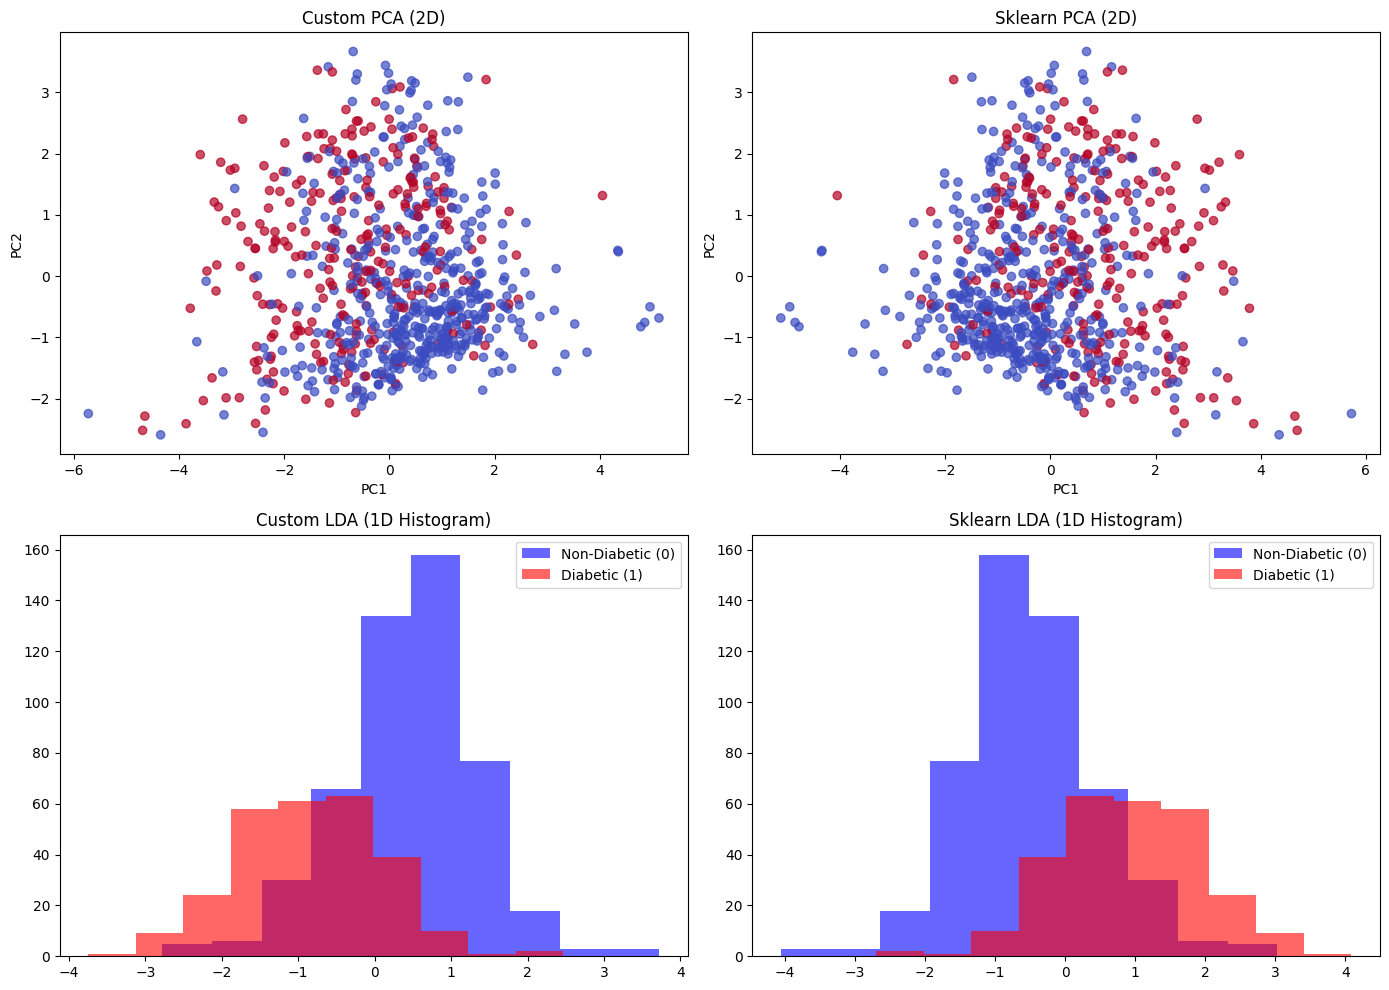
\includegraphics[width=.88\textwidth]{images/pca_lda_comparison.png}
\captionof{figure}{مقایسه دقیق خروجی‌های پیاده‌سازی دستی (\lr{Custom}) و کتابخانه‌ای (\lr{Sklearn}) برای الگوریتم‌های \lr{PCA} و \lr{LDA}}
\label{fig:pcalda_cmp}
\end{center}

\begin{itemize}
\item **تحلیل معکوس شدن علامت در محورها (\lr{Sign Inversion}):** 
همان‌طور که در نمودار \lr{PCA} و هیستوگرام \lr{LDA} مشهود است، شکل کلی پراکندگی داده‌ها در پیاده‌سازی دستی و اسکلی‌رن کاملاً یکسان است، با این تفاوت که جهت محور افقی (\lr{PC1}) معکوس ($180^\circ$ چرخش) شده است. این موضوع از نظر ریاضی کاملاً طبیعی است؛ زیرا بردارهای ویژه ($\mathbf{v}$) تنها تا ضریب یک ضرب‌کننده منفی ($\pm \mathbf{v}$) یکتا هستند و هر دو جهت از نظر حفظ واریانس معتبرند.

\item **تحلیل عدم تفکیک‌پذیری در PCA:**
در نمودارهای دو بعدی \lr{PCA} (تصاویر بالا)، داده‌های افراد دیابتی (قرمز) و غیردیابتی (آبی) به شدت در یکدیگر تداخل دارند. علت این امر عدم استفاده \lr{PCA} از برچسب داده‌هاست؛ این الگوریتم صرفاً جهتی را انتخاب می‌کند که بیشترین پراکندگی (واریانس) را داشته باشد، نه جهتی که بهترین تفکیک کلاس را ایجاد کند.

\item **تحلیل جدایش در LDA:**
در هیستوگرام‌های یک‌بعدی \lr{LDA} (تصاویر پایین)، توزیع دو کلاس به میزان قابل‌توجهی از هم تفکیک شده‌اند. مرکز توزیع بیماران غیردیابتی و دیابتی در دو سمت مخالف محور قرار گرفته‌اند که نشان‌دهنده موفقیت \lr{LDA} در بیشینه کردن فاصله میانگین کلاس‌ها نسبت به واریانس درون‌کلاسی است.
\end{itemize}
}

\field{جمع‌بندی}{
در این بخش، صحت پیاده‌سازی ریاضی الگوریتم‌های \lr{PCA} و \lr{LDA} اثبات گردید. تحلیل بصری خروجی‌ها نشان داد که جهت‌گیری بردارهای ویژه می‌تواند تفاوت علامت جزئی داشته باشد اما رفتار کلی داده‌ها یکسان است. همچنین مشخص گردید برای مسائل دسته‌بندی و جداسازی کلاس‌ها، روش با نظارت \lr{LDA} کارایی به مراتب بالاتری نسبت به روش بدون نظارت \lr{PCA} ارائه می‌دهد.
}

\end{stepbox}